
\documentclass[12pt]{amsart}
\usepackage{textcomp}

\addtolength{\hoffset}{-2.25cm}
\addtolength{\textwidth}{4.5cm}
\addtolength{\voffset}{-2.5cm}
\addtolength{\textheight}{5cm}
\setlength{\parskip}{0pt}
\setlength{\parindent}{15pt}

\usepackage{graphicx}
\graphicspath{ {./images/} }

\pagestyle{plain}

\usepackage{amsthm}
\usepackage{amsmath}
\usepackage{amssymb}

\usepackage[colorlinks = true, linkcolor = black, citecolor = black, final]{hyperref}

\usepackage{graphicx}
\usepackage{multicol}
\usepackage{ marvosym }
\usepackage{wasysym}

\usepackage{outlines}
\usepackage[utf8]{inputenc}
\usepackage[english]{babel}

\usepackage{enumitem,amssymb}
\newlist{todolist}{itemize}{2}
\setlist[todolist]{label=$\square$}
\usepackage{pifont}
\newcommand{\cmark}{\ding{51}}%
\newcommand{\xmark}{\ding{55}}%
\newcommand{\done}{\rlap{$\square$}{\raisebox{2pt}{\large\hspace{1pt}\cmark}}%
\hspace{-2.5pt}}
\newcommand{\wontfix}{\rlap{$\square$}{\large\hspace{1pt}\xmark}}

\newcommand{\pr}[1]{\left(#1\right)}

\usepackage{xcolor}
\definecolor{forestgreen}{RGB}{1, 97, 89}
\definecolor{green}{RGB}{0, 150, 0}
\definecolor{yellow}{RGB}{218, 165, 32}

\usepackage{tikz}
\usetikzlibrary{patterns}
\usetikzlibrary{arrows.meta}

\newcommand{\ds}{\displaystyle}

\setlength{\parindent}{0in}

\pagestyle{plain}

\begin{document}

\bigskip
\bigskip
\bigskip
\bigskip
\begin{titlepage}

   \begin{center}
       \vspace*{1cm}

       \textbf{\Large{An in-depth discussion on topics in neuroscience for those that might still be interested\\
       \smallskip }}

       \vspace{0.5cm}
        December 19$^{th}$, 2022
            
       \vspace{1cm}

       \textbf{By Jackson Powell\\ For Angela}
\vspace{1.5cm}
        
\centerline{\rule{13cm}{0.4pt}}
\tableofcontents
\centerline{\rule{13cm}{0.4pt}}
            
       \vspace{0.8cm}
     
       \end{center}


\begin{center}

    ``Once you know the way broadly, you can see it in all things." - Musashi Miyamoto
    
\end{center}

\end{titlepage}

\pagebreak




{\scshape J. Powell} \hfill {\scshape \large Topics in Neuroscience} \hfill {\scshape Fall, 2022}
 
\smallskip

\hrule
\bigskip
\normalsize 

\section{The Basics of Neuron Structure and Function}
\subsection{What do neurons do?} The incredibly complex functions of neurons can be summarized surprisingly well as simple wires connecting different parts of our body. Like a wire bridging a battery and an illuminated LED on a breadboard, neurons can take stimuli and elicit a response. 


\subsection{Morphology}

\subsubsection{Soma} The soma is the cell body of the neuron. This is where the nucleus (which contains DNA) resides. Many of the imporant cell functions will occur here, like transcription of genes. 

\subsubsection{Dendrites} The dendrites grow off of the cell body and form tree-branch like structures. The degree of branching, and or the complexity of the dendrites is highly dependent on the type of neuron. The dendrites most often where input signals will be delivered. Neurons will link to the dendrites of other neuron's in order to send messages. 

\subsubsection{Axon} The axon is akin to a tree's trunk. It grows off of the soma and extends a great distance away. The axon, like the dendrites, is very specific to the type of neuron. Some axons are bidirectional (bipolar) where as many are unidirectional (unipolar). The axon is a highway for electrical messages to be sent long distances. The sciatic nerve's axon, as an example, is typically longer than 1 meter. Information from your extremities will typically be routed through three neurons before reaching higher order processing in the brain---which is simply to say that neurons help information move long distances very quickly. 

\subsubsection{Synapse/terminal} The end of the axon features an axon terminal. This is known as the synapse, and it is the location at which information from one neuron \textit{synapses} onto the next. For example, you may want to contract your biceps. To do this, a neuron will have the signaling molecule acetylcholine stored in its axon terminal. This will then be released on to the dendrites of another neuron. This neuron will recieve the acetylcholine and then respond appropriately by contracting your biceps. 


\subsection{The membrane} The membrane of a neuron is like that of any other cell. We will not go too in-depth here, but there are some things worth mentioning. It is composed of a lipid bilayer, meaning the inside of the membrane will be hydrophobic (nonpolar), while the exterior will be hydrophilic (polar). The relevance of this being that polar items may not pass through the membrane due to poor interactions with the interior of the wall, while nonpolar items can more freely pass through. Hence, polar items require ion channels, transporters, and other methods to move about the membrane. \newline

The lipid composition of the membrane is also very strictly controlled. An important thing to know regarding this is that the hydrophobic heads of the lipids on the outside monolayer of the membrane (thus, those facing the extracellular space) are most often neutral in charge---they are still polar, though. Those on the inner monolayer (the cytoplasmic side) have a higher proportion of negatively charged heads. This helps create a partial membrane voltage and is incredibly important for how transmembrane proteins orient themselves in the membrane. We won't discuss that here, though. 

\section{Ion Channels and bit of Biochemistry}
\subsection{What is an ion channel?} An ion channel can be best thought of as a pore in the membrane formed by a protein. Why do we need structured pores in the membrane? Because ions can not pass directly through a membrane. Ions have a charge, meaning they are polar and can not enter the hydrophobic bilayer. Thus, channels for ions need to exist. Allowing ions to cross between cells is an essential part of life. 

\subsubsection{A common misconception} If is often said that ion channels always pass ions "with their concentration gradient." While "transporters" pass ions or molecules against their gradient. In fact, even my graduate biochemistry professor, the co-director of the biochemistry program at the University of Pennsylvania, made this same simplifying remark. But this is not true!\newline 

For example: there are many "inward rectifying potassium channels," meaning they pass potassium ions into the cell (a famous example being the Kir family of channels). Importantly, the concentration of K$^+$ outside of the cell will \underline{never} exceed the concentration inside the cell. Therefore, any and all inward pointing K$^+$ channels will inherently be "against the concentration gradient." And certainly, if the cell makes them, they must do something! How, then, does this happen if there is no active transport? Simply put: it is simply due to the random flow of ions. If an ion floats randomly about and happens to get sucked into a channel, it will pop out the other side and have no way to go back in the opposite direction. 

\subsection{Types of ion channels (with emphasis on gating)}
\subsubsection{Voltage gated ion channels} A voltage gated ion channel is one that opens depending on the voltage of the membrane it resides in. For example, there are certain voltage gated calcium channels (VGCCs) that only open when the voltage is very positive, emblematic of the peak of an action potential. What purpose does this have in a cell? Naturally, in the case of VGCCs, it ensures that certain cellular functions only occur after an AP has been delivered, like release of neurotransmitters from the synapse. \newline

You may ask yourself "how does an ion channel know when the voltage is positive or negative?" Structure informs us of almost every puzzle in biology, and this case is no different! Let us consider one potassium channel called KvAP. KvAP is hypothesized to be voltage gated due to the presence arginine side chains (as positively charged amino acid)\footnote{Ruta \textit{et al}. 2005, \textit{Cell}}. Because of the positive charge on arginine, you can imagine that if the outer membrane voltage becomes especially negative, it will pull the arginines outward, almost like opening the lid of the channel. \newline

Notably, the vast majority (but not all) of voltage gated channels open at positive voltages. This is straightforward because the resting voltage is negative, so if channels were open at negative voltages it would mean they would be active when the neuron is supposed to be "at rest." This will be discussed more in depth in the AP section. 



\subsubsection{Ligand gated} A ligand is a signaling molecule. Some channels open in response to a molecule binding to it. One essential use for this type of channel is to kickstart the action potential process. If all channels were perfectly voltage gated, then the membrane potential would never change! Ligand gated channels are responsible for the initial swings in voltage that allow for more channels to open, which further change the voltage. An example are nicotinic receptors. This is the ligand gated channel that is at the neuromuscular junction. Acetylcholine binds to nicotinic receptors from the prior neuron and cause a voltage swing, which allows more channels to open, and then eventually cause the motor neuron to fire an AP, thereby flexing the muscle. 


\subsubsection{Jackson's favorite channel: HCN}
\subsection{A note on specificity}
\subsection{A note on transporters}


\section{The Action Potential (AP)}

\subsection{Electrophysiology terms to know} First, lets begin by discussing some terms: 

\subsubsection{Conductance} Conductance is similar to the current of an individual ion across the entire membrane, and it is represented by the symbol $g_x$ where $x$ is the ion referred to. A ion that has very many open ion channels on the membrane is said to have a high conductance, while one that has few channels has low conductance. 


\subsubsection{Electric Potential (Reversal Potential)} The electric potential is similar to describing the voltage of a single ion and is represented by $E_x$. If you were to remove all other molecules, and only $x$ remained, $E_x$ is what the total membrane voltage would be. This is what determines the direction in which an ion would prefer to flow. For this reason, it is also called the \textit{Reversal Potential}, because if the membrane voltage is equal to an ion's $E$, there will be no net flow of this ion. $E$ can be calculated in the following way: 

\medskip

\begin{center}
    
    $E_x = \frac{RT}{zF}ln(\frac{[x]_{out}}{[x]_{in}})$
    
\end{center}

\medskip

Where $R$, $T$, $z$, and $F$ are constants. And $[x]$ is the concentration either inside or outside of the membrane.

\subsubsection{Resting Voltage} The resting voltage of a membrane is where it levels off to at equilibrium. If enough time passes, and there is no input signal into the membrane, it will reach said resting voltage. This can be calculated in the following way: 

\medskip

\begin{center}

    $V = \frac{g_1E_1 + g_2E_2 + ... + g_kE_k}{g_1 + g_2 + ... + g_k} = \frac{\sum_{n=1}^k g_nE_n}{\sum_{n=1}^k g_n}$
    
\end{center}

\medskip

Where $k$ is the total number of different ions considered in your system. In effect, it is the weighted average of the electric potentials of all ions around the membrane. Most often the only conductance/potential pairings that are considered are for $Na^+$ and $K^+$, because those are the highest in concentration and have orders of magnitude more of an effect on the membrane than other ions, such as $Ca^{2+}$.


\subsection{The resting state} When the membrane is at rest, how does the intracellular and extracellular ionic composition look? There is a few important things to note first:

\begin{outline}[enumerate]
\1 The membrane will be electroneutral
\1 The osmolarity should be approximately equal on a cell-to-cell level

\end{outline}

\subsection{Where do ions go, and why?} The simple way in which you can tell which direction an ion will go is with the formula: $v - E_x$. If this result is very positive, it means the ion wants to exit the cell, and if it is negative, it will want to enter the cell. Let us consider a practice example!: 

\bigskip
\begin{center}

    Let's assume $[K]_{out} = 5mM$ and $[K]_{in} = 150mM$\\
    \smallskip
    $E_k = \frac{RT}{zF}ln(\frac{[x]_{out}}{[x]_{in}}) \rightarrow 60log_{10}(\frac{[5]_{out}}{[150]_{in}}) \rightarrow \approx -88 mV$\\
    \smallskip
    
\end{center}

\bigskip

 The resting membrane potential of a neuron is approximately $-60mV$. Therefore, $v - E_k = 28mV$. Because 28 is positive, it means $K^+$ ions want to leave the cell, and will do so whenever potassium ion channels start to open up.  

\subsection{Changes are small and local} An incredibly common misconception with regard to action potentials is that the ion flux is great, and that is what drives the membrane voltage change. However, this is absolutely untrue! Let's consider an example to show this: 

\bigskip


    The capacitance of a cell ($C$) is around $1\mu F/cm^2$. If the radius of the cell is $10\mu m$, the total capacitance is:

\begin{center}

    $C_{total} = C_m \times 4\pi r^2$

\end{center}

    The movement of charge, $q$, can be calculated as:
    
\begin{center}

    $q = C_{total}\Delta V$

\end{center}

    The change in $V$ of an AP is approximately $100mV$, so:

\begin{center}

    $q = 1.3 \times 10^{-12}C$

\end{center}

    Dividing this number by Faraday's constant, $F$, gives moles, $m$. You can divide the moles by the volume to approximate $\Delta C$:

\begin{center}

    $\Delta C = \frac{m}{4\pi r^3 /3} \rightarrow 3.2 \times 10^{-7} mM$
    
\end{center}

\bigskip

If the concentration of potassium is around $150mM$, this $3.1 \times 10^{-7} mM$ is representative of a negligible change in concentration. 

\subsection{Change in concentration at the growth cone} In order that we may apply this to the growth cone we get an r value of approximately $1.75 \mu m$, and I am interested in finding the change in concentration that is capable of increasing the voltage by approximately $15mV$, indicative of reaching the threshold: 

\bigskip

\begin{center}

    $C_{total} = 10^{-6} F/cm^2 \times 4\pi (0.000175cm)^2$

    $m = q/F = (3.8 \times 10^{-13}F \times 0.015V) / 96500 C/mol$

\end{center}

\bigskip

    Thus, we get:

    \bigskip
    
\begin{center}

    $\Delta C = \frac{5.99\times10^{-20}}{4\pi (0.000175cm)^3 /3} \rightarrow 2.7 \times10^{-9} M$
    
\end{center}

\bigskip

In other words, the change in concentration required for a growth cone to rise by $15mV$ is $\approx$ 2-3$nM$.  



\subsection{Sodium} Sodium is the primary positive ion outside of the membrane, maintained around 150nM, depending on the source. An interesting hypothesis regarding this nature is that, as life originated in the ocean, it is thought that organisms adapted to pump $Na^+$ out, and this persisted to when organisms moved on land.  
\subsection{Potassium} Potassium is the primary positive intracellular ion, maintained around 120nM, depending on the source. Very few proteins use $K^+$ as a binding partner or ligand, which makes developing potassium sensors very hard. 
\subsection{Calcium} Calcium is maintained in very low concentrations inside of the cell (close to 100nM in the cytosol if I recall?), and in slightly higher concentrations in $Ca^{2+}$ stores (close to 5mM within the ER, if I recall?). Calcium is the binding partner of many proteins, making $Ca^{2+}$ sensors very easy to develop. For example, GCaMP is a fusion of calmodulin and GFP. 
\subsection{What may cause an AP?}
\subsection{Refractory period}
\subsection{Properties of APs}
\subsubsection{Bidirectional AP}
\subsubsection{Backwards AP}
\subsubsection{Successive APs}
\subsection{Physical properties of neurons that affect APs}
\subsection{Axon diameter}
\subsection{Myelination}


\section{AP Causes (In More Depth)}
\subsection{A fascinating case study: HCN}
\subsubsection{The heart} Almost all cells use voltage gated Na$^+$ channels in order to initiate an AP, but the heart is an exception. In the case of cardiac pacemaker cells, the HCN channel is used to generate action potentials. Pacemaker cells almost completely lack Na$^+$ conductance, and certainly do not have any voltage gated sodium channels. 

\subsubsection{The neuron}

\section{Hodgkin-Huxley} 

\subsection{The main form} The pair won the nobel prize for this model, which formed the basis of our understanding of action potentials. Beyond neurons, it was used in modeling pacemakers of the heart, and muscle cell depolarizations before better models existed.  The basis is simply Kirchoff's law: 

\bigskip

\begin{center}

    $C\dot{V} = I - I_{Na} - I_{K} - I_{Leak}$
    
\end{center}

\bigskip

Because the equations can be found in nearly any textbook\footnote{Izhikevich, \textit{Dynamical Systems Neuroscience}} or Wikipedia page, I will focus on some of the conceptual understanding I had issues with at first. The complete equation they Hodgkin and Huxley arrived at is as follows: 

\bigskip

\begin{center}

    $C\dot{V} = I - \bar{g}_{Na}m^3h(V - E_{Na}) - \bar{g}_{K}n^4(V - E_{K}) - \bar{g}_{L}(V - E_{L})$
    
\end{center}

\bigskip 

There are a few main points to make here. Firstly, that this model considers only 3 currents. $Na$ and $K$ are self explanatory, but $Leak$ is emblematic of the small amount of current that will always occur in cells due to the many routes of charged particles passing through the membrane.\newline

\subsection{Gating and conductance} The $\bar{g}$ represent the maximal conductance of these ions. But, shouldn't conductance be variable, depending on how many channels are open? Yes, that is what $m$, $h$, and $n$ are for. These three variables are effectively kinetic fits of the opening and closing dynamics of sodium and potassium channels. Again, I will not mention these equations explicitly as they can be found anywhere. But conceptually, there are three things to know:\newline

Firstly, $m$ is an activation curve for sodium, and the power to the 3rd represents that there are three activation gates. $h$ is an inactivation gate for sodium. Potassium has 4 activation gates $n$, and no inactivation gate. Gating can be any number of things, for example, $h$ could be a conformtional change that occurs in the channel after it has been open for $0.1 ms$ that closes it again. Naturally, the gating for every channel will be different. Because the $Leak$ current is a tonic occurance, it will not have "gating" per se.\newline

Secondly, $m$, $h$, and $n$ all are between 0 and 1 and represent the \textbf{proportion of channels open}. For instance, if $n = 1$, then 100\% of potassium channels will be open. This is why we multiply by the maximal conductance.\newline

Thirdly, $m$, $h$, and $n$ are dependent upon voltage, which affords them a time constant $\tau$. This is the conceptually most difficult part. The experimental explanation may be beneficial in understanding. Hodgkin and Huxley realized that these three gating variables will converge to different values depending on the voltage. This makes sense, because we know potassium channels are voltage gated, we would expect the gating variable $n$ to converge to around 1 as the voltage increases. But, the rate at which channels open and close is different. Therefore, their experiments were done to vary the voltage and determine how long it took the conductance of the channels to converge to some value. Does this make sense? In simplest terms: channels open and close at different rates, and that depends on the voltage.\newline

What is the implication of this? Again, look up the exact equations if you are interested. Otherwise, trust the following: $m$ has a time constant $\tau_m$ which is very small compared to $\tau_h$ and $\tau_n$. Meaning, sodium channels will open the fastest in response to a voltage increase, causing depolarization of the cell. After some delay, sodium channel inactivation ($h$) and potassium channel activation ($n$) will kick in, causing repolarization and then hyperpolarization. 

\subsection{These are all derivatives} One of the most difficult conceptual understandings I had was that $\dot{V}$, $m$, $h$, and $n$ are all rates that depend on different time constants, which take voltage as their input. So, the derivative of voltage depends on the derivative of $m$, $h$, and $n$, which depend on voltage. The cyclic nature of this makes it strange, but still doable. Use the general form of derivative, $x_{i+2} = x_{i+1} + (x_{i+1} - x_i)/t$, follow the math, and you will survive.

\section{Fitzhugh-Nagumo Reduction}

\subsection{Why would we simplify this system?} Reduction implies we are reducing the amount of variables. But why would we do this? The system is already incredibly generalized. We only consider two ion channels and are looking at a static neuron. How can we be accurate if we simplify this system any further?\newline

Let's start by doing a simple thought experiment regarding the previous model: 

\bigskip

\begin{center}

    $C\dot{V} = I - \bar{g}_{Na}m^3h(V - E_{Na}) - \bar{g}_{K}n^4(V - E_{K}) - \bar{g}_{L}(V - E_{L})$
    
\end{center}

\bigskip

As mentioned, $m$, $h$, and $n$ have their own time constants $\tau_{m,h,n}$. That means you'll need to do at least 6 calculations in order to determine $\dot{V}$, which, because it is a derivative, has its own time constant $\tau_v$. Thus, the whole equation is $4^{th}$ dimensional with respect to time and requires at least 7 or so calculations per time step. If you'd like to simulate an action potential for around 10ms with a time step of 0.01ms, that means you'll perform around 7,000 calculations. Which is not so bad!\newline 

However, let's say you want to attempt a propagating action potential. Many people would model this on an infinitely long neuron/wire, but for the sake of this thought experiment let's say you're just interested in a $1cm$ neuron/wire for $10ms$. To account for this spatial consideration, you'll need to add in another term besides $I$ which receives  current input from the previous segment of the neuron. So this brings us up to at least 8,000 calculations.\newline

You'd probably want to divide up the neuron into segments on the order of $1\mu m$. This multiplies our 8,000 calculations by an additional 100,000, giving us 800,000,000 to worry about. Still, this is not horrendous. But, this considers a 1D wire. Neurons are 3D dimensional. We are already considering a system that is $4^{th}$ dimensional with respect to time, and now we desire to consider $3^{rd}$ dimensional with respect to space. Imagine trying to calculate the flux through a $1000 \times 1000 \times 1000$ resolution box (i.e., perhaps $\mu m^3$ with good resolution). The surface area of this box is thus $6\times 10^6$. Now extend this surface area to include the length of the wire and the area of the soma and dendrites, giving you thousands of millions of points to calculate per time iteration. And, we are still only considering two ion channels. Neurons have dozens and dozens of channels all with different gating kinetics. It does not consider things like lateral inhibition, birufcation, dendritic input, etc. I'll not bother telling you how many calculations we need to perform beyond this point---but it would be large. 

\subsection{What do we do about it?} What do we know about the time constants mentioned in the previous section? Roughly speaking, some are fast and some are slow. The upswing of an action potential is on a fast time constant, and the repolarization is on a slow time constant. We also know that the upswing portion is roughly a positive feedback loop, so as voltage increases, so should the derivative of voltage.\newline

This helps us arrive at least at the following: 

\bigskip

\begin{center}

    $\dot{V} = V \times f(x)$
    
\end{center}

\bigskip

Simply meaning that the derivative should scale with voltage in some way. We also know that there are at least two "equilibrium points" in a neuron. Meaning, when the neuron is at rest, the $\dot{V}$ will be zero. And, when the neuron reaches the peak of the action potential, the same is true. This will allow us to immediately assume something interesting:

\bigskip

\begin{center}

    $\dot{V} = V(V - V_{rest})(V - V_{max})$
    
\end{center}

\bigskip

We are already almost there. What we have just done is said that when either $V = V_{rest}$ or $V = V_{max}$, the $\dot{V}$ will not change. These are all on the aforementioned "fast" time scale, and as this is representative of the activation of the action potential, it is effectively a simplification of the sodium channel dynamics. This is also extremely easy to measure experimentally.\newline

On our second time scale, the slow time scale, we have the inactivation/repolarization function. How will this look like? Just as with the first equation, we will want this curve to increase in magnitude with voltage. Because $n$ represented the potassium channel activation in the previous segment, we can use that as our repolarization function here. 

\bigskip

\begin{center}

    $\dot{n} = V - \gamma n$
    
\end{center}

\bigskip

What does this say? It says that our repolarization curve $\dot{n}$ will increase with respect to voltage. But, it will also decrease with respect to itself according to some scaling factor $\gamma$\newline

Now we have reduced our function down to two dimensions and can combine terms: 

\bigskip

\begin{center}

    $\dot{V} = V(V - V_{rest})(V - V_{max}) - n$\\
    $\dot{n} = V - \gamma n$
    
\end{center}

\bigskip

But, we still want voltage to be affected by an injected current, so we can simply add this term back in. And it is also in this equation that we will add our spatial dependence to reach the following: 

\bigskip

\begin{center}

    $\dot{V} = I_{app} + [V(V - V_{rest})(V - V_{max}) - n] +  D\frac{\partial V^2}{\partial x^2}$\\
    
\end{center}

\bigskip

$D$ is our spatial dependence, which represents the diffusion of charge around the neuron membrane. And that's it, for now! 

\section{Ion Channel General Forms}

\section{Calcium Dynamics}

\subsection{Overarching Equation} As with the previous ideas, the compounded equation is a summation of the currents generated by calcium flux equating to $dCa / dt$.\newline

Here she is: 

\begin{center}

    $\frac{dCa}{dt} = D_c\frac{\partial^2 Ca}{\partial x^2} + J_{ipr} + \frac{G_{circ}}{G_{CSA}}(J_{in} - J_{pm}) + J_{RyR} - J_{ser} - J_{on} + J_{off}$

\end{center}

\bigskip

To briefly go over this, we are solving for the chance in $Ca$ concentration. $D_c$ is a diffusion coefficient term multiplied against the second derivative of the calcium concentration with respect to time. $G_{circ} / G_{CSA}$ is the circumference of the growth cone over the growth cone's cross sectional area. This is multiplied by $J_{in}$ minus $J_{pm}$, which are the flux of calcium into and out of the cell respectively. Naturally, $J_{in}$ will be contributed to by Piezo. $J_{RyR}$ is the flux of calcium out of the ER, and $J_{ser}$ is the flux into the ER as set by the SERCA pump. $J_{on}$ and $J_{off}$ is the binding and unbinding of calcium to buffers. Gorgeous and simple in this form, but of course, each variable comes with its own model. Let's discuss below: 

\subsection{Buffers} $J_{on}$ and $J_{off}$ are simplified greatly under a few assumptions. The first being that we can assume the buffer concentration is high and greatly exceeds that of the calcium concentration, therefore calcium binding to the buffer does not change the total buffer concentration in any meaningful way. Secondly, we assume that buffer binding is fast enough to be considered instant (or rather, on a time scale much faster than that which we are differentiating with). In this way:

\begin{center}

    $J_{on} = k_+cb_t$\\
    $J_{off} = k_-b$\\
    $\frac{\partial b}{\partial t} =  k_+cb_t - k_-b$
    
\end{center}
\bigskip

Where $k_+$ is the binding rate constant, $c$ is the concentration, $b_t$ is the total concentration of buffer, $k_-$ is the unbinding rate constant, and $b$ is the concentration of bound buffer. Not so bad! You could also include the concentration of buffer as changing via diffusion under the  equation: $D_b(\partial^2 b / \partial t^2)$. In this instance, I think it is fair to simply assume that the buffer is saturating the growth cone, and therefore it is not relevant to include its flow rate.\newline

\subsubsection{Buffer Testing} With the knowledge that the number of moles per division is $4\times10^{-12} nmol/div
$, I began by testing the scenario when there was no $k_+$ at all. Once this was tuned to cause the cell to approach a concentration 100 times that of the resting state, the concentration of unbound could be properly tuned so that the resting state be the desired number of moles.\newline

Some progress has been made, but evidently this will be a more daunting task than described above. A large consideration is the concentration of calcium being multiplied by the $k$ of binding.\newline

This round of testing revealed a remarkable amount of issues, in fact.


\subsection{RyR Flux} RyR flux can be written in a number of says, such as the following\footnote{\url{https://www.frontiersin.org/articles/10.3389/fphys.2012.00114/full\#F1}}: 

\bigskip

\begin{center}

    $J_{ryr} = N_{ryr}(g_{ryr}/v_D)(C_{er} - C_{cyt})$
    
\end{center}

\bigskip

Where $v_D$ is the dyadic space volume, $g_{ryr}$ is the RyR channel conductance, $C_{er}$ is the concentration inside the ER, $C_{cyt}$ is the concentration in the cytoplasm, and $N_{ryr}$ is he stochastic number of RyR channels. This is not sufficient, yet, as it describes the movement of calcium only in response to a gradient and not using RyR channel kinetics or, most importantly, calcium activation. You'll notice there is no reference to the opening and closing kinetics, and is more similar to something like the $g_L$ which you would se in the Hogdkin-Huxley model.\newline

This covers things like leak. To include calcium activation, we will want to use something like this\footnote{Note: there seems to be an issue with $\dot{w}$ in the equations below. It seems that $w$ will be hard clamped to 1 due to the power with which the cytosolic $Ca^{2+}$ concentration is. Need to fix this.}: 

\bigskip
\begin{center}

    $J_{ryr} = (v_{rel}P_{open} + v_{leak})(C_{er} - C_{cyt})$\\
    \smallskip
    $P_{open} = \frac{w(1 + C^3_{cyt} / K_b)}{K_a / C^4_{cyt} + 1 + C_{cyt}^3/ K_b}$\\
    \smallskip
    $\dot{w} = \frac{w_{\infty} - w}{\tau_w}; w_{\infty} = \frac{K_a / C^4_{cyt} + 1 + C_{cyt}^3/ K_b}{1/K_c + K_a / C^4_{cyt} + 1 + C_{cyt}^3/ K_b}; \tau_w = w_{\infty}/K_d$
    
\end{center}

And for $J_{ser}$:

\begin{center}

    $J_{ser} = v_{ser}\frac{C^2_{cyt}}{C^2_{cyt} + K^2_P}$\\
    
\end{center}

\bigskip

 $J_{ser}$ is the Hill function, where $v_{ser}$ is the max velocity and $K_P$ is the half max velocity. The values are measured in prior papers\footnote{\url{https://www.ncbi.nlm.nih.gov/pmc/articles/PMC1233835/?page=1}}. There are complaints to be made about this function, though. It is, like many starter models, quite an oversimplification. In fact, it has even been shown that the SERCA pump can reverse in direction if the ER concentration gets too high, and therefore produces ATP in the process. \newline

 A better version would be: 

 \bigskip

 \begin{center}

    $J_{serca} = \frac{c^2 - K_1K_2K_3K_4K_5K_6c_e^2}{\alpha_1c^2 + \alpha_2c_e^2 + \alpha_3c^2c^2_e + \alpha_4}$
     
 \end{center}

 \bigskip

 All of the kinetic values refer to the different states the SERCA pump may be in. The $\alpha$ values refer to rate functions. One can make many simplifying assumptions regarding the kinetics, such as assuming that binding and unbinding occurs at maximal rates. This takes the very complex $\alpha$ equations and replaces them with corresponding $\beta$ functions, but maintains the same form as the original equation. For the purposes of a relatively multiplexed model already, I find it not super useful to use this in-depth version of the SERCA pump, and will instead use the Hill model most likely.

 
\subsection{Spatial Dealings} The most clear way to heal with the spatial component, to me, is to calculate the amount of moles of Ca$^{2+}$ in each cube, then use that to calculate the total moles.\newline


\bigskip

\begin{center}
    $\frac{120\mathrm{nM}}{\mathrm{L}} \cdot \frac{\mathrm{L}}{1000\mathrm{mL}} \cdot {\frac{4}{3}\pi(0.000\mathrm{2cm})^3} \cdot 6.022\times 10^{23} \approx 2400$ molecules\\
\end{center}


\bigskip

I am taking this to be: 

\bigskip

\begin{center}
    $\frac{120nM}{L}\frac{L}{1000mL}\frac{4/3\pi(0.0002cm)^3}{\# of divisions} = 4\times10^{-12} nmol/div$\\
    This equates to: 
    $2,400 \: molecules / \# \: of \: div$
\end{center}

\bigskip

Meaning that there is approx 6 molecules of $Ca^{2+}$ in a 20 $\times$ 20 box.

\subsection{Diffusion} Diffusion is accomplished using some diffusion coefficient. In the \textbf{Overarching Equation} this is stated as $D_c$. This value can be tuned however desired. The important bit is the second derivative of $Ca$ with respect to space. This is done simply in the general form of a second derivative, as written below: 

\begin{center}

    $f'' = \frac{f_{x - 1} - 2f_x + f_{x + 1}}{x^2}$
    
\end{center}

\bigskip

In this case, you can simply say that $x$ is one division, and therefore ignore the denominator. I don't recall if I mentioned this elsewhere, but one may wonder how one would solve for an edge case, as the general form of a second derivative requires three data points. The solution is that it is simply the first derivative of the non-edge side. That is, since the second derivative is the difference in derivatives, that leaves simply the derivative of one side minus zero.\newline

Evidently, this method has some slight issues in which the $[Ca^{2+}]$ can occasionally go negative. How this occurs, I am unsure. But this can be avoided explicitly using some other methods, which will perhaps be discussed later. 


 \section{Piezo Itself Try 1}

 \subsection{A Good Model} The rule of a good model is to, before writing any code whatsoever, determine some testable hypotheses. Models make predictions about the world, and if done well, reveal which values are most measurable to validate or invalidate the predictions. As Snyed once said, if someone asks you why you didn't test \textit{this} or \textit{that}, you can safely ignore their comments, as they do not understand the purpose of modeling. So on that note, what are some hypotheses we have regarding Piezo?:\newline

On $Ca^{2+}$ release: 
\begin{enumerate}
    \item Hypothesis 1: Piezo alone

    Firstly, it is possible that Piezo alone is the primary driving force for $Ca^{2+}$ change within the growth cone. This possibility likely manifest itself in very small concentration changes in calcium as a result of Piezo opening. 
    
    \item Hypothesis 2: Piezo with help

    Another possibility, one which I lean toward at this moment, is the release of $Ca^{2+}$ through RyR channels of the ER that are in the growth cone. This would likely result in larger swings in $Ca^{2+}$ concentration. Experimentally, this is easily testable. 
\end{enumerate}

\bigskip

 There is a question of why $Ca^{2+}$ influx does not trigger action potentials which propagate down the axon in C3da., So, on membrane potential: 
\begin{enumerate}
    \item Hypothesis 1: Negligible

   One possibility is that the calcium influx is so low that it does not cause a meaningful change in membrane voltage. I would say that this is unlikely, as was shown in the section \textbf{(Changes are small and local)}. 
    
    \item Hypothesis 2: Clamped

    More plausible, to me, is that the membrane voltage is being clamped via some kind of outward rectifying potassium channels, namely KCa3.1. Experimentally, this is easily testable. 

    \item Hypothesis 3: Diffusion

    It diffuses away fast.
\end{enumerate}

\bigskip



On Piezo activation: 
\begin{enumerate}
    \item Hypothesis 1: Growth cone

   The physical movement of the growth cone as it attempts to grow is a possible Piezo activator. As exocytosis occurs, but the volume of the cell stays the same, it will cause the membrane to become more rigid and therefore modulates Piezo.  
    
    \item Hypothesis 2: Glia

    It has been shown that ECM environment grabs onto outgrowths of dendrites and activate mechanosensitive ion channels in \textit{C. elegans}\footnote{\url{https://www.cell.com/developmental-cell/pdf/S1534-5807(22)00376-8.pdf}}. It is plausible too then that the same thing occurs via glia-Piezo interactions. 
\end{enumerate}


\subsection{Experimental Verification} Experiments that can be used to corroborate or refute the model include: 

 \begin{enumerate}
 \item NO imaging (as a proxy of Piezo activation)
     \item Ca$^{2+}$ imaging (new GCaMP seems very powerful)
     \begin{itemize}
         \item If need be, patch-clamp is also an option
     \end{itemize}
     \item Atomic force microscopy (AFM) \textit{in vivo}
     \item Growth of neurons on different substrates
     \item FRET to measure force
     \item FRAP to measure membrane fluidity
     \item Axon injury both 
     \begin{itemize}
         \item \textit{in vivo} in \textit{Drosophila} or Mice
         \item \textit{in vitro} with cultured neurons
     \end{itemize}
 \end{enumerate}

\subsection{Activation Overview} There are many considerations regarding Piezo activation. We can consider force-from-lipids, which may include things like membrane stretch, compression, or shear. Similarly, another consideration is the fluidity of the membrane. We can consider force-from-proteins, which may involve direct binding of membrane proteins from glia to neurons, which manipulate the membrane. The seemingly stochastic flipodia out-pushing could include all of these interactions. For the sake of this model, it would be best to attempt a few alternative hypotheses, which may explain Piezo activation. For example, we can scan a multitude of membrane fluidities, pressures, etc. and determien which has the biggest affect on Piezo activation. There is also the issue of substrate stiffness, which too may affect Piezo (in this case, this will be analagous to the stiffness of the glia membrane).\newline 

\subsection{Voltage Gating} Piezo is voltage gated\footnote{\url{https://www.nature.com/articles/s41467-018-03502-7}}. One can debate the importance of this in general systems. This paper shows half-max activation close to 100 mV. The few cells that may be able to get there are likely to have more to worry about than Piezo (namely the conductance of VGCCs). \textit{Drosophila} Piezo is said to have voltage gating that is much more similar to a standard VGCC. Therefore, we can use the following sigmoid formalism as a contributor to Piezo activation: 

\bigskip


\begin{equation} \label{eq8}
\begin{split}
P_V = \frac{1}{\exp\pr{\pr{100 - V}/20} + 1}
\end{split}
\end{equation}

\bigskip

The units being in $mV$. However, I think that even this is not necessary, as it will only be relevant during an action potential, which, in our case, does not occur. 

\subsection{Pressure Gating} Pressure gating is likely the most relevant of the pack. $30mmHg$ seems to be the most accurate half-max pressure\footnote{\url{https://www.sciencedirect.com/science/article/pii/S0968000421000220\#bb0270}}\footnote{\url{https://www.science.org/doi/full/10.1126/science.1193270?casa_token=gKZRiU1R_vAAAAAA\%3AAuhBFZP-QjXckn7G9aBL6A_ZJfCjsRrUIqoXCbBA1887i29wPWtzlMBfdwShr45kBM7Pj-N4NYVlfEQ}}. We can again consider a sigmoid curve as follows: 


\begin{equation} \label{eq8}
\begin{split}
P_P = \frac{1}{\exp\pr{\pr{30 - P}/7} + 1}
\end{split}
\end{equation}

\bigskip

The units being in $mmHg$, of course. This is an unavoidable consideration. 

\subsection{Substrate Stiffness} Substrate stiffness is also extremely important. In this case, a Gaussian distribution is appropriate, with values centered on our data as follows: 

\bigskip

\begin{equation} \label{eq8}
\begin{split}
P_S = \frac{1}{0.25\sqrt{2 \pi}}\exp\pr{\frac{1}{2}\pr{\pr{S - 0.7}/0.25}}^2
\end{split}
\end{equation}


\bigskip

The units, in this case, are $kPa$. It is difficult to discern the correct standard deviation. This was selected in order to encompass the $0.3kPa-1.0kPa$ range we saw. 

\subsection{Closing/Inactivation} The time constant, $\tau$, values for Piezo vary greatly in both organism and type. As some papers show $6$ms\footnote{\url{https://www.nature.com/articles/nature10812}}, and others $16$ms\footnote{\url{https://www.science.org/doi/full/10.1126/science.1193270?casa_token=WnOGIrz8PbAAAAAA\%3AdA422PZ9tigaVHLD6IxvFlWpQer0KOFm_jvCrohrhgnSzzdEPOXhZo_koo-cZeWbLeNSTFPtSJ3bdtA}} for Piezo1 for $\tau$. Therefore, the general form of inactvation is $\exp(t / \tau)$. The units being ms. Therefore, if a cluster of $N$ channels opens at time $t_0$, and $\tau = 10$ms, at time $t_{10}$ there should be $\approx 0.368 \times N$ still open.  

\subsection{Unification} The simplified, general form of Piezo opening and closing is: 

\bigskip

\begin{equation} \label{eq8}
\begin{split}
N_{open} = P_{total} \times N_{closed} - P_{close}\times N_{open}
\end{split}
\end{equation}

\bigskip

It is likely that voltage can open Piezo independent of the other parameters. I would suspect that the substrate stiffness, however, is a contributor to opening rather than a controller. Therefore, we will multiply the probability of the substrate stiffness to that of the pressure applied. The stiffness of the neuron membrane is also likely very important to the pressure applied. That is, if the membrane is very fluid, no amount of pressure will activate Piezo. \\

To summarize, the membrane tension alone of the surrounding glia (the substrate) should not be sufficient to activate Piezo, and similarly, that force acted by glia on Piezo will not be effective if the membrane of the glia is especially fluid or stiff. Too, receiving that same force will not be effective if the neuron's membrane is too fluid. \\

\begin{equation} \label{eq8}
\begin{split}
P_T & = P_V + P_PP_S\\
P_{total} & = \frac{1}{\exp\pr{\pr{0.5 - P_{T}}/0.1} + 1}
\end{split}
\end{equation}

\bigskip

With $P_V$ being the probability of opening due to voltage, $P_P$ being the probability of opening due to pressure and $P_N$ being favorable probability of stiffness of the neuron, and $P_S$ being the substrate. One important liberty I am likely to take is assuming that Piezo opens almost instantly in comparison to the $dT$ value I will select, and that $\tau$ is much slower than the opening speed.\newline

% \frac{1}{e^{(\frac{100-(\frac{f(x)}{0.006})}{10})}+1}


\begin{center}
\includegraphics[width=0.8\textwidth]{Piezo_comparison.png}
\end{center}

It is certain that multiple conformations exist, particularly defining an inactive state which exists after opening, during which some structural resetting must occur. I am postulating 5 states: defined here as $N_{open1}$, $N_{open2}$, $N_{open3}$, $N_{inactive}$, $N_{closed}$. $N_{open1}$ describes ``full open" which characterizes normal activation and prefers to flow into the inactive state after. $N_{open2}$ describes when the ion channel is forced to stay open (under continuous pressure, shown in the Coste \textit{et al.} paper), despite its time constant lapsing. $N_{open3}$ was added because there is a tail region that follows $N_{open2}$ (i.e., after the continuously applied pressure stops at 600ms, there is not an immediate drop to 0 in current), implying that some final open state takes some time to close. $N_{inactive}$ means that the channels are not open, and cannot be opened for some time. $N_{closed}$ is once the channel is closed and fully ready to be opened once again. The calculations done for each, thus, are: 

\bigskip

\begin{center}
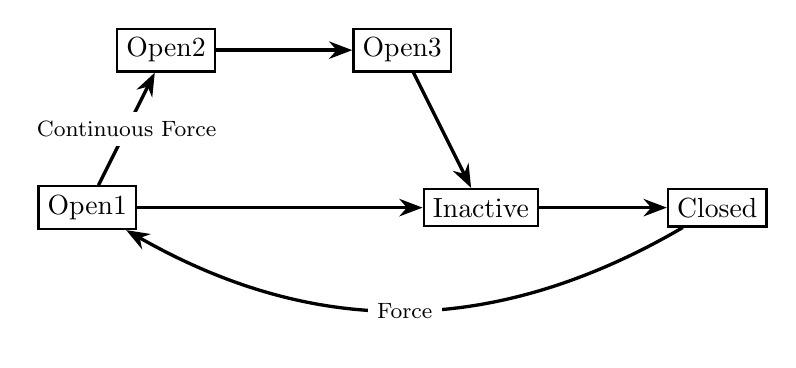
\begin{tikzpicture}
\begin{scope}[every node/.style={rectangle,thick,draw}]
    \node (A) at (0,0) {Open1};
    \node (B) at (1,2) {Open2};
    \node (C) at (4,2) {Open3};
    \node (D) at (5,0) {Inactive};
    \node (E) at (8,0) {Closed};

    \end{scope}

\begin{scope}[>={Stealth[black]},
              every node/.style={fill=white,rectangle},
              every edge/.style={draw=black,very thick}]
    \path [->] (A) edge node[pos=0.5] {\footnotesize{Continuous Force}} (B);
    \path [->] (A) edge (D);
    \path [->] (B) edge (C);
    \path [->] (C) edge (D);
    \path [->] (D) edge (E);
    \path [->] (E) edge[bend left=30] node[pos=0.5] {\footnotesize{Force}} (A); 
    
    \end{scope}

\end{tikzpicture}
\end{center}


\begin{equation} \label{eq8}
\begin{split}
N_{open1}^{i+1} &=  e^{-\Delta t / \tau_{open}}N_{open1}^{i} + P_{total}N_{closed}^{i} \\ 
N_{open2}^{i+1} &= P_{total}N_{open2}^{i} + P_{total}\pr{1-e^{-\Delta t / \tau_{open}}}N_{open1}^{i} \\ 
N_{open3}^{i+1} &=  e^{-\Delta t / \tau_{open3}}N_{open1}^{i} + \pr{1-P_{total}}N_{open2}^{i}\\ 
N_{inactive}^{i+1} &= e^{-\Delta t / \tau_{inact}}N_{inactive}^{i} + \pr{1-P_{total}}\pr{1-e^{-\Delta t / \tau_{open}}}N_{open1}^{i} + \pr{1-e^{-\Delta t / \tau_{open3}}}N_{open3}^{i}\\
N_{closed}^{i+1} &= \pr{1 - P_{total}}N_{closed}^{i} + \pr{1-e^{\Delta t / \tau_{inact}}}N_{inactive}^{i} \\
\end{split}
\end{equation}

\bigskip

I set $\tau_{open3}, \tau_{inact} \approx 100$ms, and $\tau_{open} \approx 10$ms. This agrees with experimentally recorded values for Piezo's time constant. 



\bigskip

\subsection{Failure} It brings me incredible sadness to say, but this is, in fact, completely wrong! I made the dumb mistake of assuming the data shown on the previous figure, from Coste \textit{et al}., is in the expression of Piezo alone. It is for this reason that I tried to make the Piezo model resemble this exactly. However, the continuous activation is, in fact, not at all Piezo and is instead likely some other mechanosensitive channels! Ths was shown in Fig. 2C in the same paper. One must always scroll down. I will leave all of this up for the sake of future onlookers. Notably, the previous equations can probably be re-purposed a bit. 


 \section{Piezo Itself Try 2}

 \subsection{Introduction} Let us take a moment to look at Fig. 3 of this paper\footnote{\url{https://www.nature.com/articles/nature10801}}. It seems that C4da have Piezo, and that one can hold Piezo open in C4da via continuous pressure. One mild concern with this is that they were able to separate neurons directly from the larva. I am wondering how this may have impacted e-phys. 

\subsection{Qualitative Interpretation} It seems to me that a faster rise and fall is more associated with complete activation of Piezo, that which approaches a $P_{total}$ of 1. A more bell shaped curve, that which does not have a sharp peak, is more associated with a partial activation. A linear falling edge is more associated with minimal activation, which is maintained over long periods by the activation of otherwise un-activated channel. You may wonder why this information is useful. In fact, it can be used to predict the stiffness of the membrane. That is, if one knows qualitatively the shape, and one applies a force of around  60 mmHg, then one can postulate the stiffness range based on the curve (i.e., knowing that 60 mmHg should maximize Piezo activation, if we see a pattern of a high peak, we can assume that the stiffness range compliments this Piezo activation). 


\subsection{Piezo Equations}

\begin{center}
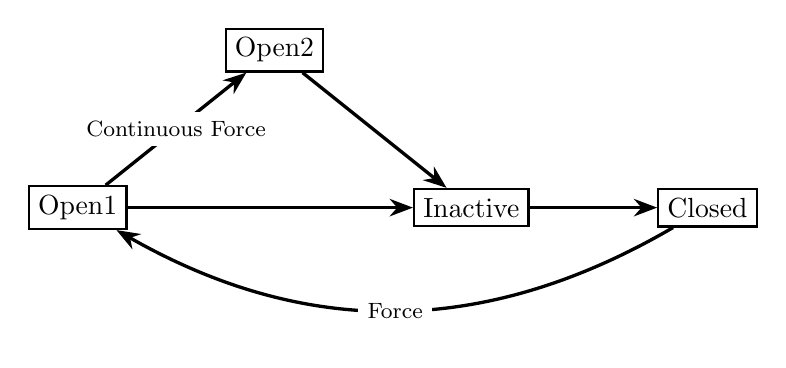
\begin{tikzpicture}
\begin{scope}[every node/.style={rectangle,thick,draw}]
    \node (A) at (0,0) {Open1};
    \node (B) at (2.5,2) {Open2};
    \node (D) at (5,0) {Inactive};
    \node (E) at (8,0) {Closed};

    \end{scope}

\begin{scope}[>={Stealth[black]},
              every node/.style={fill=white,rectangle},
              every edge/.style={draw=black,very thick}]
    \path [->] (A) edge node[pos=0.5] {\footnotesize{Continuous Force}} (B);
    \path [->] (A) edge (D);
    \path [->] (B) edge (D);
    \path [->] (D) edge (E);
    \path [->] (E) edge[bend left=30] node[pos=0.5] {\footnotesize{Force}} (A); 
    
    \end{scope}

\end{tikzpicture}
\end{center}


\begin{equation} \label{eq8}
\begin{split}
N_{open1}^{i+1} &=  e^{-\Delta t / \tau_{open}}N_{open1}^{i} + P_{total}N_{closed}^{i} \\ 
N_{open2}^{i+1} &= P_{P}N_{open2}^{i} + P_{P}\pr{1-e^{-\Delta t / \tau_{open}}}N_{open1}^{i} \\ 
N_{inactive}^{i+1} &= e^{-\Delta t / \tau_{inact}}N_{inactive}^{i} + \pr{1-P_{P}}\pr{1-e^{-\Delta t / \tau_{open}}}N_{open1}^{i} + \pr{1-P_P}N_{open2}^{i}\\
N_{closed}^{i+1} &= \pr{1 - P_{total}}N_{closed}^{i} + \pr{1-e^{\Delta t / \tau_{inact}}}N_{inactive}^{i} \\
\end{split}
\end{equation}

\subsection{Background Equations}

\begin{center}
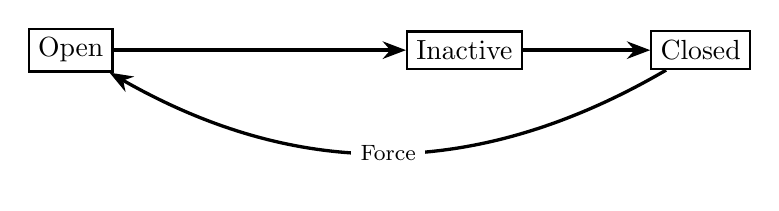
\begin{tikzpicture}
\begin{scope}[every node/.style={rectangle,thick,draw}]
    \node (A) at (0,0) {Open};
    \node (D) at (5,0) {Inactive};
    \node (E) at (8,0) {Closed};

    \end{scope}

\begin{scope}[>={Stealth[black]},
              every node/.style={fill=white,rectangle},
              every edge/.style={draw=black,very thick}]
    \path [->] (A) edge (D);
    \path [->] (D) edge (E);
    \path [->] (E) edge[bend left=30] node[pos=0.5] {\footnotesize{Force}} (A); 
    
    \end{scope}

\end{tikzpicture}
\end{center}

\begin{equation} \label{eq8}
\begin{split}
N_{open}^{i+1} &=  e^{-\Delta t / \tau_{open}}N_{open}^{i} + P_{P}N_{closed}^{i} \\ 
N_{inactive}^{i+1} &= e^{-\Delta t / \tau_{inact}}N_{inactive}^{i} + \pr{1-e^{-\Delta t / \tau_{open}}}N_{open}^{i}\\
N_{closed}^{i+1} &= \pr{1 - P_{P}}N_{closed}^{i} + \pr{1-e^{\Delta t / \tau_{inact}}}N_{inactive}^{i} \\
\end{split}
\end{equation}

\end{document}